\documentclass[12pt,a4]{article}
\usepackage[left=1.8cm,right=1.8cm,top=32mm,columnsep=20pt]{geometry}

\usepackage[utf8]{inputenc} %Formato de codificación
\usepackage[spanish, es-tabla, es-nodecimaldot]{babel}
\usepackage{amsmath} %paquete para escribir ecuaciones matemáticas
\usepackage{float} %Para posicionar figuras
\usepackage{graphicx} %Para poder poner figuras
\usepackage{hyperref} %Permite usar hipervínculos
\usepackage{multicol} %Para hacer doble columna
\usepackage[sorting=none]{biblatex} %Imports biblatex package. To cite use \cite{reference_label}
\usepackage{csquotes}

\title{Informe de Física: Encontrando el coeficiente de fricción dinámica}
\author{Francisco Carruthers, Facundo Firpo y Joel Jablonski\\ [2mm]
\small \texttt{\{fcarruthers, ffirpo, jjablonski\}@udesa.edu.ar}\\
\small Fisica I, tutorial Vinograd}
\date{2do Semestre 2024}


\begin{document}

\maketitle

\begin{abstract}
    Utilizando un carrito, una soga y una polea, se busca encontrar el coeficiente de fricción dinámica entre el carrito y la superficie. Para ello, se mide la aceleración del carrito con distintas masas y se calcula el coeficiente de fricción dinámica. También, utilizamos varias superficies para ver cómo afecta el coeficiente de fricción.
\end{abstract}

\section{Introducción}

(Descripción del experimento)

(Desarrollo de Newton y Vinculos del problema)

\begin{table}
    \centering
    \begin{tabular}{|c|c|}
        \hline
        \textbf{Objeto} & \textbf{Masa(g)} \\
        \hline
        Pesa dorada & $72 \pm 1$ \\
        Pesa plateada & $23 \pm 1$ \\
        Pesa madera & $6 \pm 1$ \\
        Trineo & $109 \pm 1$ \\
        Metro & $134 \pm 1$ \\
        \hline
    \end{tabular}
    \caption{Mediciones de masa}
    \label{tab:mediciones}
\end{table}

\newpage
\section{Calibración}

Utilizamos un sistema de referencia para calibrar el sistema.

\begin{figure}[H]
    \centering
    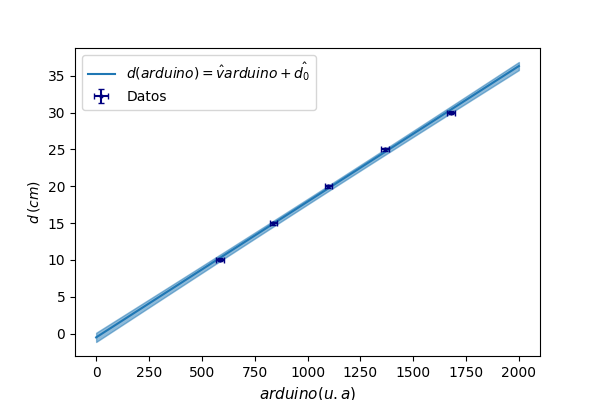
\includegraphics[width=0.9\linewidth]{Calibracion.png}
    \caption{Calibración del sistema}
    \label{fig:calibracion}
\end{figure}

Pendiente: $0.0184 \pm 0.0005$ \\

Ordenada al origen: ($-0.5 \pm 0.5$) cm\\

Distancia para 600: ($10.5 \pm 0.4$) cm \\

\newpage

\section{Resultados}

\subsection{Posicion}

\subsubsection*{Madera y Trineo}

En un primer caso dejamos el trineo deslizar sobre la mesa de madera. \\

\begin{figure}[H]
    \centering
    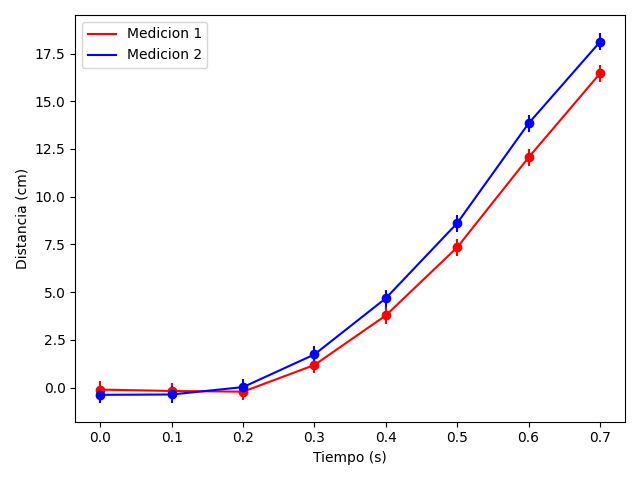
\includegraphics[width=0.4\linewidth]{TiempoVsDistanciaPisoMadera2PB_O.png}
    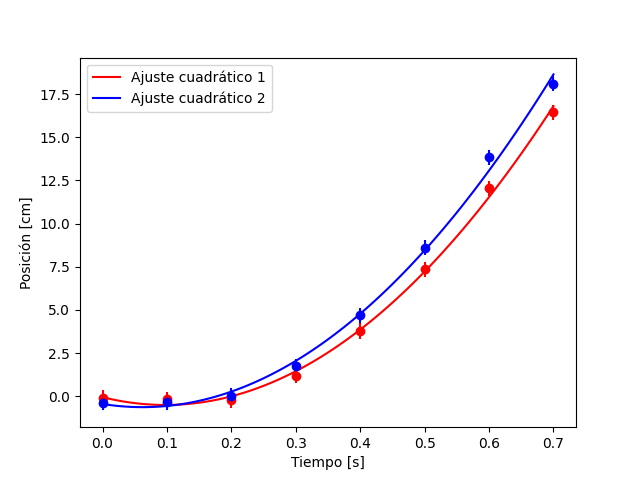
\includegraphics[width=0.44\linewidth]{ajuste2_PisoMadera2PB_O.png}
    \caption{$M = 161 \pm 1 g, m = 72 \pm 1 g$}
    \label{fig:2PB_O piso trineo}

\end{figure}

\begin{figure}[H]
    \centering
    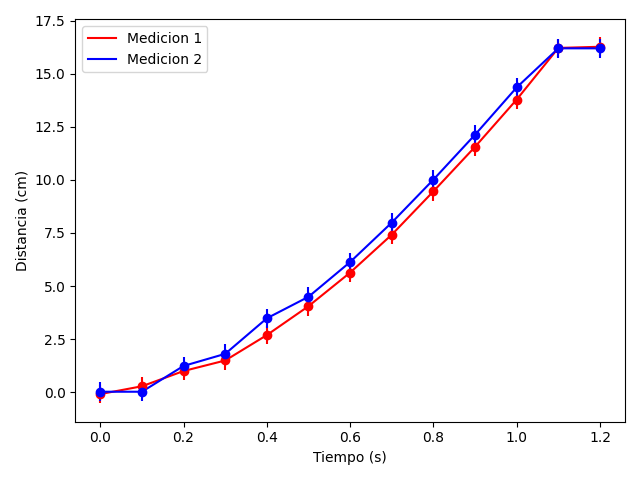
\includegraphics[width=0.4\linewidth]{TiempoVsDistanciaPisoMaderaMPB_O.png}
    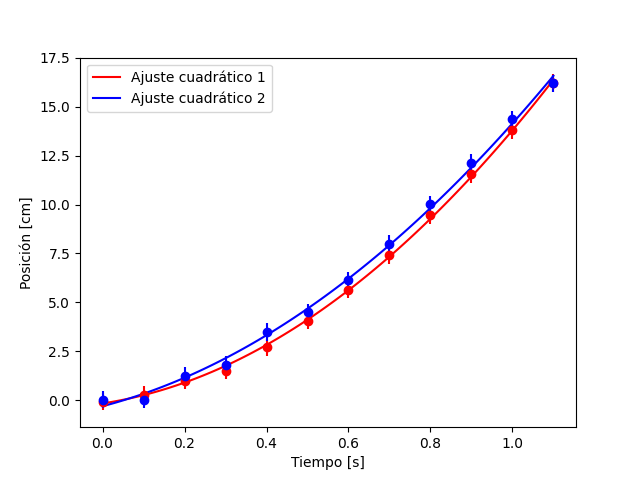
\includegraphics[width=0.44\linewidth]{ajuste2_PisoMaderaMPB_O.png}
    \caption{$M = 243 \pm 1 g, m = 95 \pm 1 g$}
    \label{fig:M_OP piso trineo}
\end{figure}

\begin{figure}[H]
    \centering
    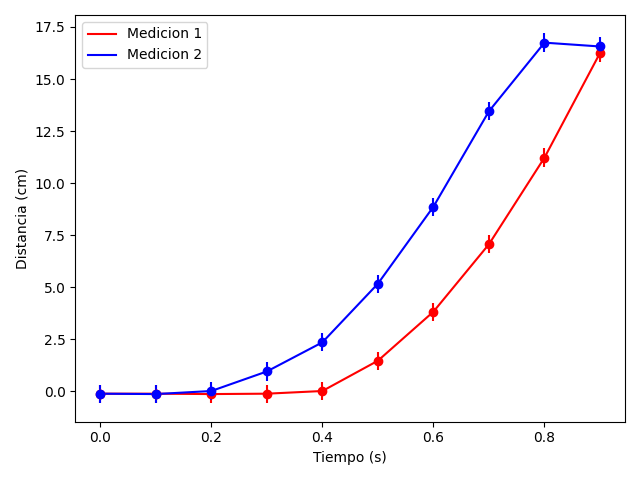
\includegraphics[width=0.4\linewidth]{TiempoVsDistanciaPisoMaderaV_2P.png}
    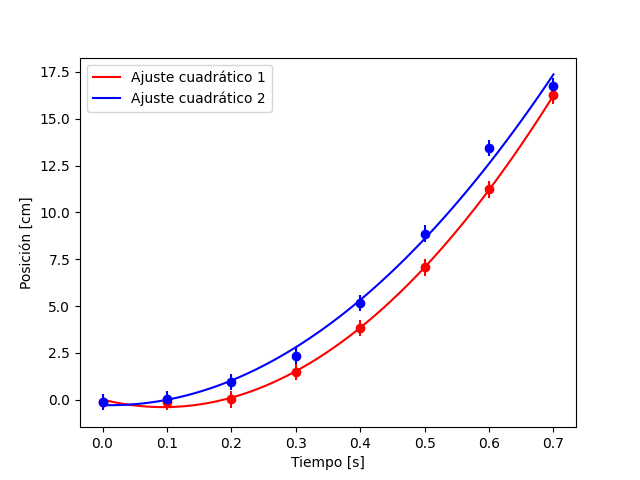
\includegraphics[width=0.44\linewidth]{ajuste2_PisoMaderaV_2P.png}
    \caption{$M = 109 \pm 1 g, m = 46 \pm 1 g$}
    \label{fig:V_2P piso trineo}
\end{figure}


Vemos en las figuras \ref{fig:2PB_O piso trineo} y \ref{fig:M_OP piso trineo} que ambas mediciones se parecen bastante entre si en cada caso pero que en \ref{fig:V_2P piso trineo} hay una diferencia en la pendiente. Esto nos va a llevar a que la incerteza del $\mu_d$ sea grande.

\subsubsection*{Papel y trineo}

Luego, le pegamos papel a la mesa y repetimos el experimento.

\begin{figure}[H]
    \centering
    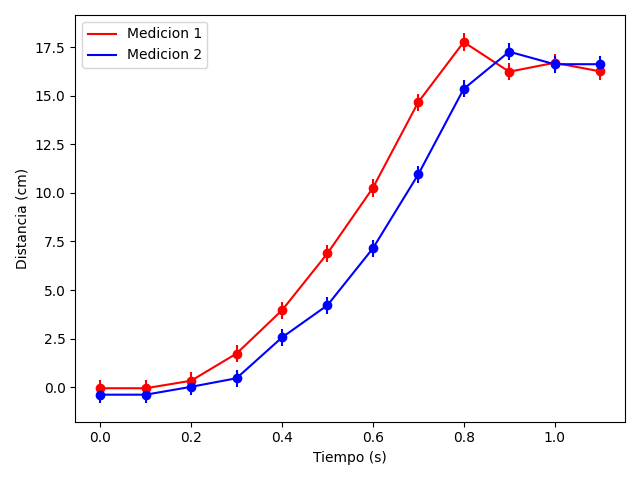
\includegraphics[width=0.4\linewidth]{TiempoVsDistanciaPisoHoja2PB_O.png}
    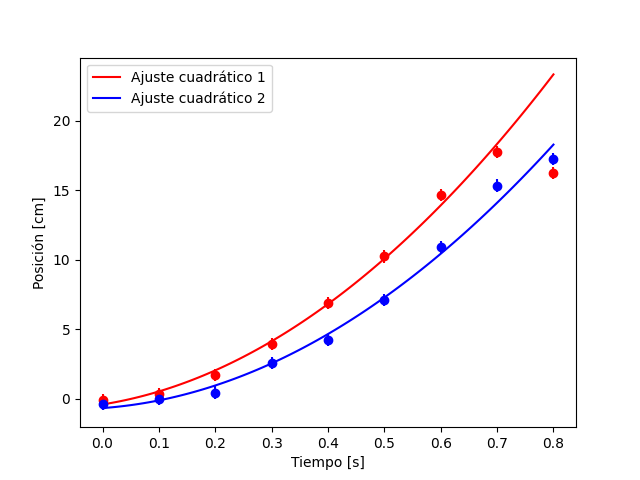
\includegraphics[width=0.44\linewidth]{ajuste2_PisoHoja2PB_O.png}
    \caption{$M = 161 \pm 1 g, m = 72 \pm 1 g$}
    \label{fig:2PB_O piso hoja}
\end{figure}

\begin{figure}[H]
    \centering
    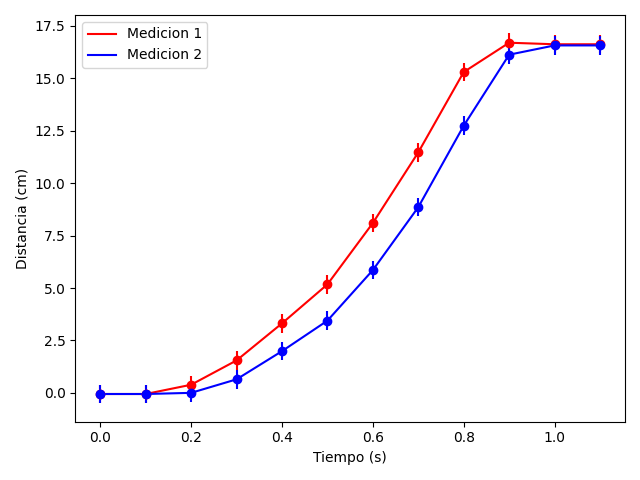
\includegraphics[width=0.4\linewidth]{TiempoVsDistanciaPisoHojaM_OP.png}
    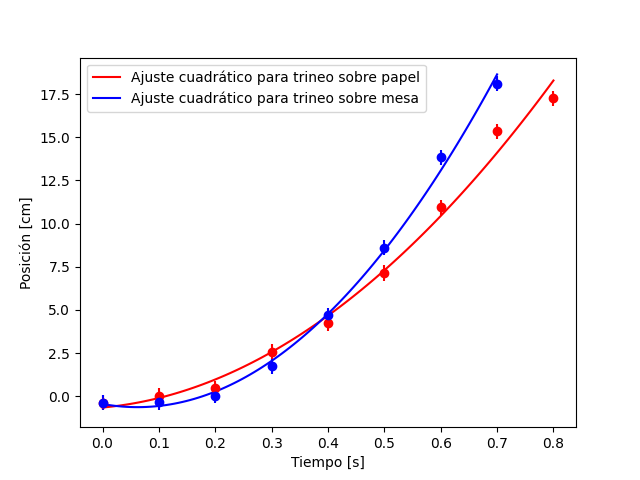
\includegraphics[width=0.44\linewidth]{ajuste2_PisoHojaM_OP.png}
    \caption{$M = 243 \pm 1 g, m = 95 \pm 1 g$}
    \label{fig:M_OP piso hoja}
\end{figure}

\begin{figure}[H]
    \centering
    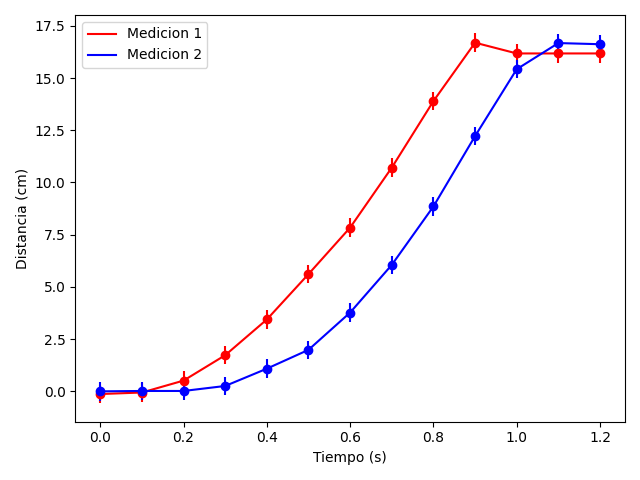
\includegraphics[width=0.4\linewidth]{TiempoVsDistanciaPisoHojaV_2P.png}
    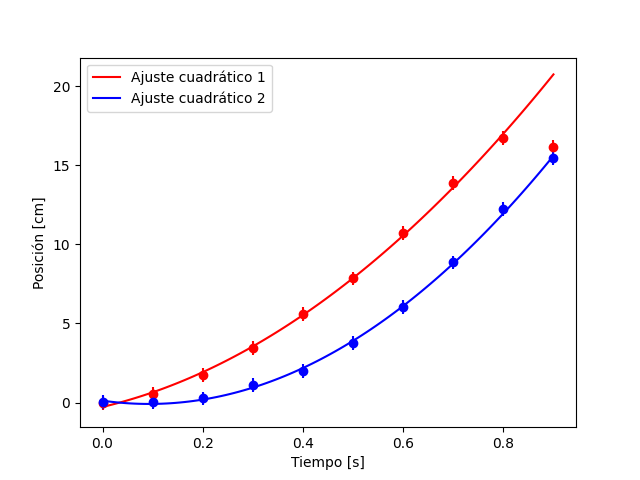
\includegraphics[width=0.44\linewidth]{ajuste2_PisoHojaV_2P.png}
    \caption{$M = 109 \pm 1 g, m = 46 \pm 1 g$}
    \label{fig:V_2P piso hoja}
\end{figure}

Vemos que en las figuras \ref{fig:2PB_O piso hoja} y \ref{fig:M_OP piso hoja} las pendientes son muy parecidas, pero en \ref{fig:V_2P piso hoja} hay una diferencia en la pendiente. Esto nos va a llevar a que la incerteza del $\mu_d$ sea grande.

\subsubsection*{Papel y Papel}

Por ultimo, pegamos otro papel al trineo y repetimos el experimento.

\begin{figure}[H]
    \centering
    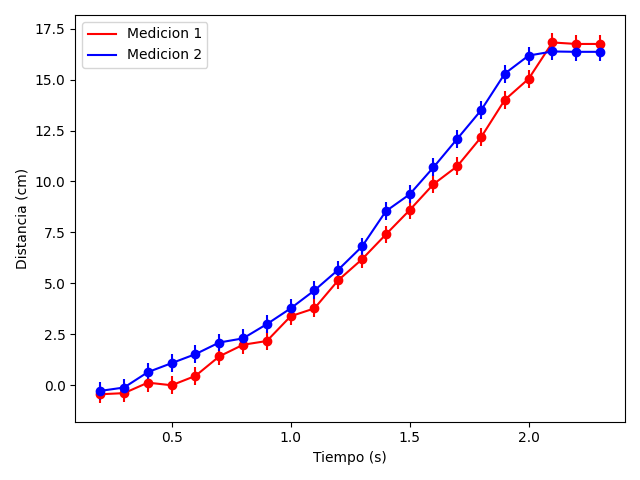
\includegraphics[width=0.4\linewidth]{TiempoVsDistanciaPapelPapelM_O.png}
    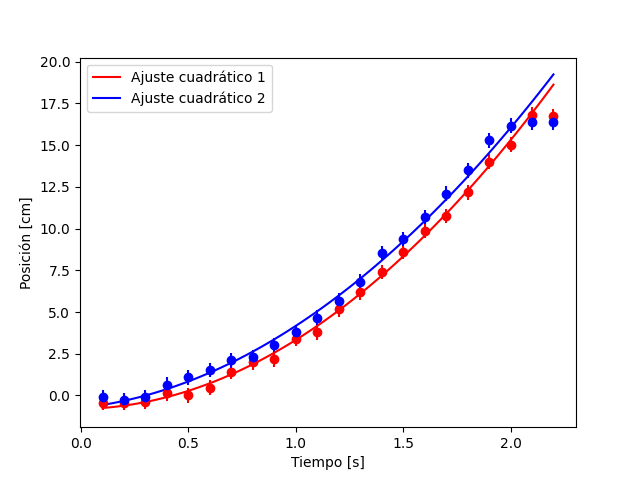
\includegraphics[width=0.44\linewidth]{ajuste2_PapelPapelM_O.png}
    \caption{$M = 243 \pm 1 g, m = 72 \pm 1 g$}
    \label{fig:M_O papel papel}
\end{figure}

\begin{figure}[H]
    \centering
    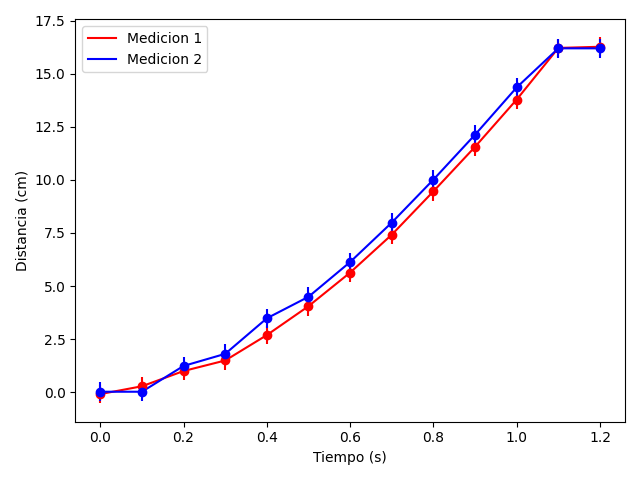
\includegraphics[width=0.4\linewidth]{TiempoVsDistanciaPapelPapelM_OP.png}
    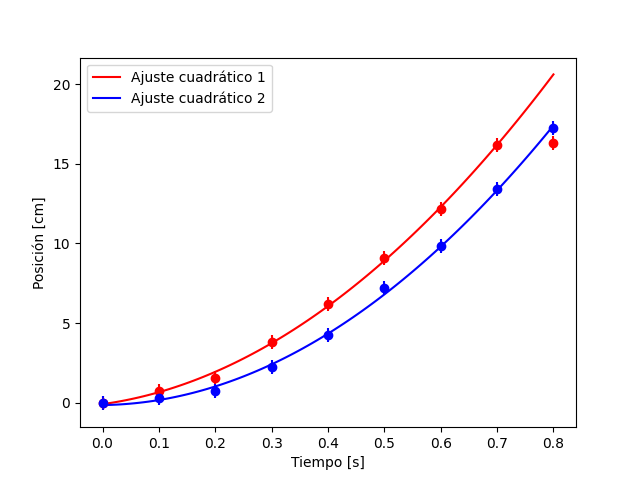
\includegraphics[width=0.44\linewidth]{ajuste2_PapelPapelM_OP.png}
    \caption{$M = 243 \pm 1 g, m = 95 \pm 1 g$}
    \label{fig:M_OP papel papel}
\end{figure}

\begin{figure}[H] %check esto
    \centering
    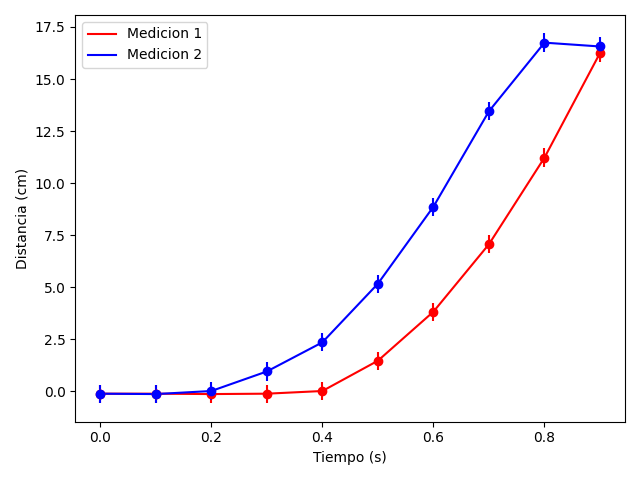
\includegraphics[width=0.4\linewidth]{TiempoVsDistanciaPapelPapelV_O.png}
    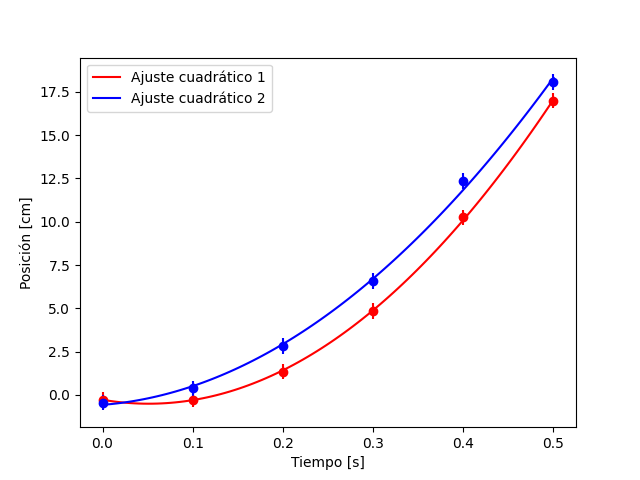
\includegraphics[width=0.44\linewidth]{ajuste2_PapelPapelV_O.png}
    \caption{$M = 109 \pm 1 g, m = 72 \pm 1 g$}
    \label{fig:TvDV_O papel papel}
\end{figure}

\subsection{Obtencion del $\mu_d$}

\begin{figure}[H]
    \centering
    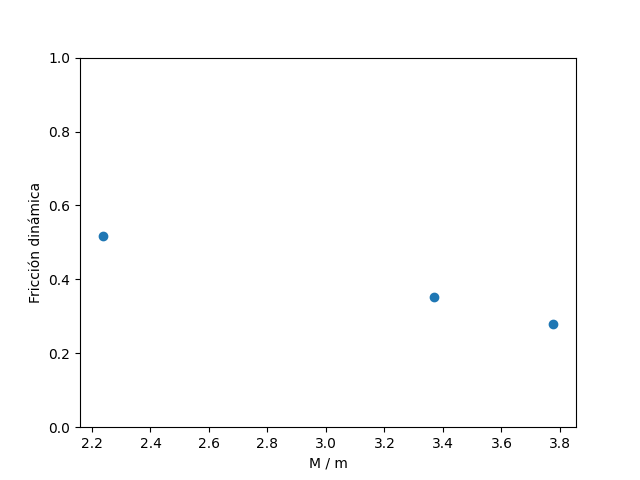
\includegraphics[width=0.6\linewidth]{ud_PisoMadera.png}
    \caption{Madera y trineo}
    \label{fig:mu_d piso trineo}
\end{figure}

\begin{figure}[H]
    \centering
    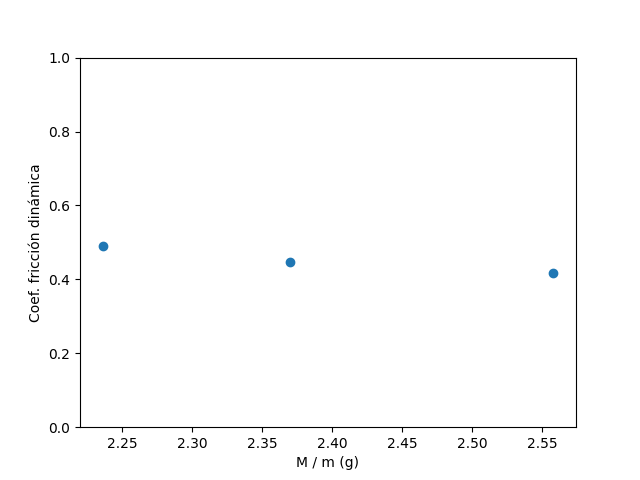
\includegraphics[width=0.6\linewidth]{ud_PisoPapel.png}
    \caption{Papel y trineo}
    \label{fig:mu_d piso hoja}
\end{figure}

\begin{figure}[H]
    \centering
    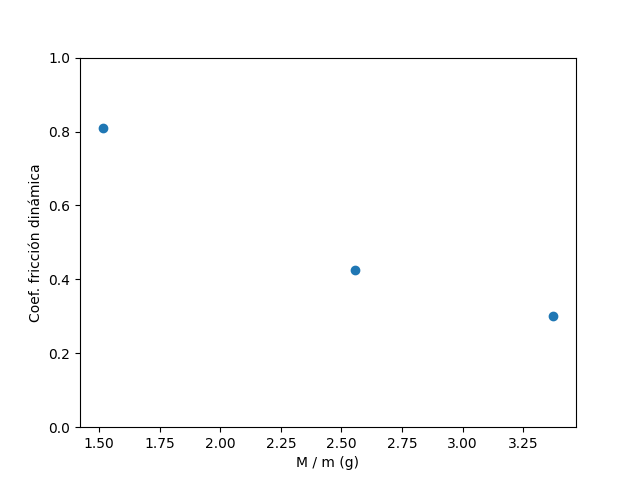
\includegraphics[width=0.6\linewidth]{ud_PapelPapel.png}
    \caption{Papel y papel}
    \label{fig:mu_d papel papel}
\end{figure}

Sacando un promedio de los valores obtenidos en las figuras \ref{fig:mu_d piso trineo}, \ref{fig:mu_d piso hoja} y \ref{fig:mu_d papel papel} obtenemos un valor de $\mu_d$ para cada superficie.

\begin{figure}[H]
    \begin{minipage}{0.5\textwidth}
        \centering
        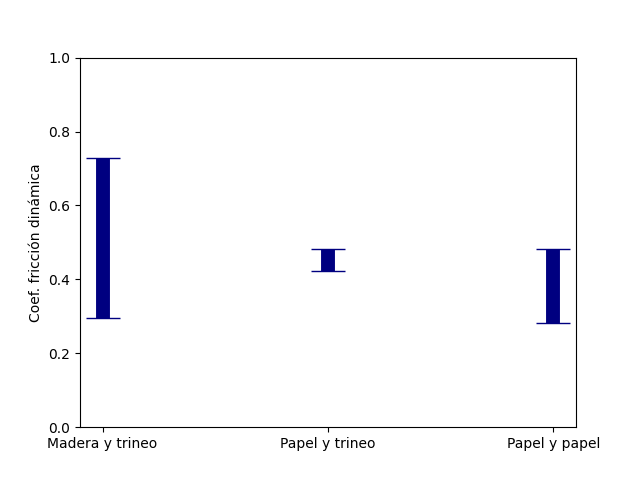
\includegraphics[width=0.9\linewidth]{ud_Combined.png}
        \caption{Promedio de $\mu_d$ para cada superficie}
        \label{fig:mu_d promedio}
    \end{minipage}\hfill
    \begin{minipage}{0.5\textwidth}
        \centering
        \begin{table}[H]
            \centering
            \begin{tabular}{|c|c|}
                \hline
                \textbf{Superficie} & \textbf{$\mu_d$}\\
                \hline
                Madera y trineo & $0.4 \pm 0.1$\\
                Papel y trineo & $0.45 \pm 0.03$ \\
                Papel y Papel & $0.5 \pm 0.2$ \\
                \hline
            \end{tabular}
            \caption{Valores de $\mu_d$ y sus incertezas para cada superficie}
            \label{tab:mu_d}
        \end{table}
    \end{minipage}
\end{figure}

\section{Conclusiones}

En conclusión, este experimento ha logrado cumplir con los objetivos planteados de determinar el coeficiente de fricción dinámica entre un carrito y diferentes superficies utilizando métodos experimentales. A través de las mediciones de aceleración en diversas configuraciones de masa y superficie, se obtuvieron valores para el coeficiente de fricción dinámica $\mu_d$, destacándose variaciones significativas entre las diferentes superficies analizadas, como madera, papel sobre madera, y papel sobre papel.

Los resultados obtenidos evidencian que la fricción varía no solo en función de la masa sino también de la textura de las superficies en contacto. Por ejemplo, el valor de $\mu_d$ en la superficie de madera fue de 0.4 ± 0.1, mientras que en papel sobre papel fue mayor, alcanzando un promedio de 0.5 ± 0.2. Esta variación en el coeficiente es indicativa de la influencia de la rugosidad y la naturaleza del material en la interacción de fricción.

La incertidumbre en los resultados, sobre todo en algunas mediciones, refleja la necesidad de tener en cuenta las posibles fuentes de error en los experimentos, como la calibración de los instrumentos. Sin embargo, los valores obtenidos permiten confirmar que las diferencias observadas en las superficies afectan significativamente la dinámica del movimiento del trineo.

En definitiva, este trabajo ha permitido no solo calcular el coeficiente de fricción dinámica, sino también comprender la importancia de las condiciones experimentales y cómo pequeñas variaciones pueden impactar en los resultados, reforzando el valor de una correcta medición y calibración en estudios físicos.


\end{document}